根据上一节中的信息,您现在可以使用LLVM库创建自己的项目。下面几节介绍一种名为Tiny的小型语言,这个项目将称为tinylang。尽管本节中的工具只是一个“Hello, world”,但它的结构与实际编译器所需的所有部分一样。\par

\hspace*{\fill} \par %插入空行
\textbf{创建目录结构}

第一个问题,tinylang项目是否应该与LLVM一起构建(就像clang一样)?还是应该是一个只使用LLVM库的独立项目?前一种情况下,还需要决定在哪里创建项目。\par

首先,假设tinylang应该与LLVM一起构建。在哪里放置项目有不同的选择。第一种解决方案是在llvm-projects目录中为项目创建一个子目录。此目录中的所有项目都将作为构建LLVM的一部分使用并构建。在并行项目布局创建之前,这是标准的构建方式,例如:clang。\par

第二种选择是将tinylang项目放在顶层目录中。因为它不是一个正式的LLVM项目,所以无需让CMake知道。当运行cmake时,需要指定-DLLVM\underline{~}ENABLE\underline{~}PROJECTS=tinylang,以便在构建中包含项目。\par

第三种选择是将项目目录放在其他地方,即llvm-project目录之外。当然,需要告诉CMake关于这个位置的信息。若位置是/src/tinylang,那么需要指定-DLLVM\underline{~}ENABLE\underline{~}PROJECTS=tinylang -DLLVM\underline{~}EXTERNAL\underline{~}TINYLANG\underline{~}SOURCE\underline{~}DIR=/src/tinylang。\par

如果将项目作为独立项目构建,则需要找到LLVM库。这是在CMakeLists.txt中完成的,本节稍后将讨论这个。\par

了解了可能的选择后,哪一个最好呢?使您的项目成为LLVM源代码树的一部分有点不灵活。要是您不打算将项目添加到顶层项目列表中,建议使用一个单独的目录。可以在GitHub或类似的服务上维护,而不用担心如何与LLVM项目同步。正如前面所示,您仍然可以与其他LLVM项目一起构建它。\par

让我们用一个非常简单的库和应用程序创建一个项目。第一步是创建目录布局,假设当前位于克隆llvm-project目录。使用mkdir(Unix)或md(Windows)创建以下目录:\par

\hspace*{\fill} \par %插入空行
\begin{center}
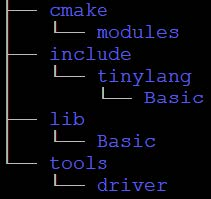
\includegraphics{content/1/chapter2/images/2.jpg}\\
图2.2 – 项目所需的目录
\end{center}

接下来,我们将构建描述和源文件放在这些目录中。\par

\hspace*{\fill} \par %插入空行
\textbf{添加CMake文件}

上一节中确认了代码的基本结构。在tinylang目录中,按照以下步骤创建一个名为CMakeLists.txt的文件:\par

\begin{enumerate}
\item 该文件首先使用cmake\underline{~}minimum\underline{~}required()来声明CMake的最低版本:
\begin{tcolorbox}[colback=white,colframe=black]
cmake\underline{~}minimum\underline{~}required(VERSION 3.13.4)
\end{tcolorbox}

\item 下一个语句是if()。如果条件为真,那么项目将独立构建,并且需要额外的设置。该条件使用两个变量,CMAKE\underline{~}SOURCE\underline{~}DIR和CMAKE\underline{~}CURRENT\underline{~}SOURCE\underline{~}DIR。CMAKE\underline{~}SOURCE\underline{~}DIR变量是在CMAKE命令行中给出的顶层源目录。正如在关于目录布局的讨论中所看到的,每个带有源文件的目录都有一个CMakeLists.txt。CMakeLists.txt所位于的当前文件夹记录在CMAKE\underline{~}CURRENT\underline{~}SOURCE\underline{~}DIR变量中。如果两个变量具有相同的字符串值,那么项目将独立构建。否则,CMAKE\underline{~}SOURCE\underline{~}DIR将是llvm目录:
\begin{tcolorbox}[colback=white,colframe=black]
if(CMAKE\underline{~}SOURCE\underline{~}DIR STREQUAL CMAKE\underline{~}CURRENT\underline{~}SOURCE\underline{~}DIR)
\end{tcolorbox}

单独设置也很简单,每个CMake项目都需要一个名称。这里,将它设置为Tinylang:
\begin{tcolorbox}[colback=white,colframe=black]
\hspace*{0.5cm}project(Tinylang)
\end{tcolorbox}

\item 搜索LLVM包,将LLVM目录添加到CMake模块路径中:
\begin{tcolorbox}[colback=white,colframe=black]
\hspace*{0.5cm}find\underline{~}package(LLVM REQUIRED HINTS \\
\hspace*{1cm}"\${LLVM\underline{~}CMAKE\underline{~}PATH}") \\
\hspace*{0.5cm}list(APPEND CMAKE\underline{~}MODULE\underline{~}PATH \${LLVM\underline{~}DIR})
\end{tcolorbox}

\item 然后,包含了LLVM提供的另外三个CMake模块。只有使用Visual Studio作为构建编译器,并设置正确的运行时库,再次链接时才需要第一个。另外两个模块添加LLVM使用的宏,并根据提供的选项配置构建:
\begin{tcolorbox}[colback=white,colframe=black]
\hspace*{0.5cm}include(ChooseMSVCCRT) \\
\hspace*{0.5cm}include(AddLLVM) \\
\hspace*{0.5cm}include(HandleLLVMOptions)
\end{tcolorbox}

\item 接下来,将LLVM头文件的路径添加到include搜索路径中。新增两个目录。添加了构建目录中的include目录,因为这里保存了自动生成的文件。另一个include目录位于源目录中:
\begin{tcolorbox}[colback=white,colframe=black]
\hspace*{0.5cm}include\underline{~}directories("\${LLVM\underline{~}BINARY\underline{~}DIR}/include" \\
\hspace*{1cm}"\${LLVM\underline{~}INCLUDE\underline{~}DIR}")
\end{tcolorbox}
 
\item 使用link\underline{~}directories(),LLVM库的路径添加到链接器中:
\begin{tcolorbox}[colback=white,colframe=black]
\hspace*{0.5cm}link\underline{~}directories("\${LLVM\underline{~}LIBRARY\underline{~}DIR}")
\end{tcolorbox}
 
\item 最后,设置一个标志来表示项目是独立构建的:
\begin{tcolorbox}[colback=white,colframe=black]
\hspace*{0.5cm}set(TINYLANG\underline{~}BUILT\underline{~}STANDALONE 1) \\
endif()
\end{tcolorbox}

\item 现在遵循常见的设置。将cmake/modules目录添加到CMake模块搜索路径中。可以添加自己的CMake模块:
\begin{tcolorbox}[colback=white,colframe=black]
list(APPEND CMAKE\underline{~}MODULE\underline{~}PATH \\
\hspace*{0.5cm}"\${CMAKE\underline{~}CURRENT\underline{~}SOURCE\underline{~}DIR}/cmake/modules")
\end{tcolorbox}
 
\item 接下来,检查用户是否正在执行超出构建树的构建。与LLVM一样,我们要求用户使用单独的目录来构建项目:
\begin{tcolorbox}[colback=white,colframe=black]
if(CMAKE\underline{~}SOURCE\underline{~}DIR STREQUAL \\  \hspace*{0.3cm}CMAKE\underline{~}BINARY\underline{~}DIR AND NOT \\ \hspace*{0.3cm}MSVC\underline{~}IDE) \\
	\hspace*{0.5cm}message(FATAL\underline{~}ERROR "In-source builds are not allowed.") \\
endif()
\end{tcolorbox}
 
\item tinylang的版本号通过configure\underline{~}file()命令写到生成文件中。版本号取自TINYLANG\underline{~}VER\allowbreak SION\underline{~}STRING ,configure\underline{~}file()命令会读取一个输入文件,用CMake变量的当前值替换它们,并写入一个输出文件。请注意,输入文件是从源目录读取的,并写入构建目录:
\begin{tcolorbox}[colback=white,colframe=black]
set(TINYLANG\underline{~}VERSION\underline{~}STRING "0.1") \\
	configure\underline{~}file(\${CMAKE\underline{~}CURRENT\underline{~}SOURCE\underline{~}DIR}/include/ \\
	\hspace*{0.5cm}tinylang/Basic/Version.inc.in \\
\${CMAKE\underline{~}CURRENT\underline{~}BINARY\underline{~}DIR}/include/tinylang/Basic/Version.inc)
\end{tcolorbox}

\item 接下来,将包含另一个CMake模块。AddTinylang模块中,有一些辅助功能:
\begin{tcolorbox}[colback=white,colframe=black]
	include(AddTinylang)
\end{tcolorbox}
 
\item 接下来是另一个include\underline{~}directories()语句。将把我们自己的include目录添加到搜索路径的开头。独立版本中,需要添加了两个目录:
\begin{tcolorbox}[colback=white,colframe=black]
include\underline{~}directories(BEFORE \\
\hspace*{0.5cm}\${CMAKE\underline{~}CURRENT\underline{~}BINARY\underline{~}DIR}/include \\
\hspace*{0.5cm}\${CMAKE\underline{~}CURRENT\underline{~}SOURCE\underline{~}DIR}/include \\
)
\end{tcolorbox}
 
\item 文件的末尾,在lib和tools目录其中找到CMakeLists.txt。这个示例应用程序只有lib和tools目录下的源文件,因此不需要其他文件。更复杂的项目将添加更多的目录,例如:单元测试:
\begin{tcolorbox}[colback=white,colframe=black]
add\underline{~}subdirectory(lib) \\
add\underline{~}subdirectory(tools)
\end{tcolorbox}
\end{enumerate}

这就完成了您的项目描述。\par

AddTinylang.make模块位于cmake/modules目录下。有以下内容:\par

\begin{tcolorbox}[colback=white,colframe=black]
macro(add\underline{~}tinylang\underline{~}subdirectory name) \\
\hspace*{0.5cm}add\underline{~}llvm\underline{~}subdirectory(TINYLANG TOOL \${name}) \\
endmacro() \\
\\
macro(add\underline{~}tinylang\underline{~}library name) \\
\hspace*{0.5cm}if(BUILD\underline{~}SHARED\underline{~}LIBS) \\
\hspace*{1cm}set(LIBTYPE SHARED) \\
\hspace*{0.5cm}else() \\
\hspace*{1cm}set(LIBTYPE STATIC) \\
\hspace*{0.5cm}endif() \\
\\
\hspace*{0.5cm}llvm\underline{~}add\underline{~}library(\${name} \${LIBTYPE} \${ARGN}) \\
\hspace*{0.5cm}if(TARGET \${name}) \\
\hspace*{1cm}target\underline{~}link\underline{~}libraries(\${name} INTERFACE  \\
\hspace*{1.5cm}\${LLVM\underline{~}COMMON\underline{~}LIBS})  \\
\hspace*{1cm}install(TARGETS \${name}  \\
\hspace*{1.5cm}COMPONENT \${name} \\
\hspace*{1.5cm}LIBRARY DESTINATION lib\${LLVM\underline{~}LIBDIR\underline{~}SUFFIX} \\
\hspace*{1.5cm}ARCHIVE DESTINATION lib\${LLVM\underline{~}LIBDIR\underline{~}SUFFIX} \\
\hspace*{1.5cm}RUNTIME DESTINATION bin) \\
\hspace*{0.5cm}else() \\
\hspace*{1cm}add\underline{~}custom\underline{~}target(\${name}) \\
\hspace*{0.5cm}endif() \\
endmacro() \\
 \\
macro(add\underline{~}tinylang\underline{~}executable name) \\
\hspace*{0.5cm}add\underline{~}llvm\underline{~}executable(\${name} \${ARGN} ) \\
endmacro() \\
 \\
macro(add\underline{~}tinylang\underline{~}tool name) \\
\hspace*{0.5cm}add\underline{~}tinylang\underline{~}executable(\${name} \${ARGN}) \\
\hspace*{0.5cm}install(TARGETS \${name} \\
\hspace*{1cm}RUNTIME DESTINATION bin \\
\hspace*{1cm}COMPONENT \${name}) \\
endmacro()
\end{tcolorbox}

包含该模块,可以使用add\underline{~}tinylang\underline{~}subdirectory()、add\underline{~}tinylang\underline{~}library()、add\underline{~}tinylang\underline{~}exe\allowbreak cutable()和add\underline{~}tinylang\underline{~}tool()函数。这些是LLVM(在AddLLVM模块中)提供的函数包装器。tinylang\underline{~}subdirectory()为构建添加了一个新的源目录。此外,还添加了一个新的CMake选项。使用此选项,用户可以控制是否应该编译目录的内容。使用add\underline{~}tinylang\underline{~}library(),可以定义库并安装。Add \underline{~}tinylang\underline{~}executable()定义了可执行文件,Add \underline{~}tinylang\underline{~}tool()定义了同样安装的可执行文件。\par

lib目录中,即使没有源代码,也需要CMakeLists.txt文件,必须包含这个项目库的源目录。打开文本编辑器,将以下内容保存在文件中:\par

\begin{tcolorbox}[colback=white,colframe=black]
add\underline{~}subdirectory(Basic)
\end{tcolorbox}

大型项目将创建几个库,源代码将放在lib的子目录中。每个目录都必须添加到CMakeLists.txt文件中。我们的小项目只有一个名为Basic的库,所以只需要一行代码。\par

Basic库只有一个源文件Version.cpp。这个目录中的CMakeLists.txt文件同样简单:\par

\begin{tcolorbox}[colback=white,colframe=black]
add\underline{~}tinylang\underline{~}library(tinylangBasic \\
\hspace*{0.5cm}Version.cpp \\
)
\end{tcolorbox}

定义了一个名为tinylangBasic的新库,并将编译后的Version.cpp添加到这个库中。LLVM选项可以控制这是一个动态库还是静态库。默认情况下,会创建静态库。\par

在tools目录中重复相同的步骤。这个文件夹中的CMakeLists.txt文件几乎和lib目录中一样简单:\par

\begin{tcolorbox}[colback=white,colframe=black]
create\underline{~}subdirectory\underline{~}options(TINYLANG TOOL) \\
add\underline{~}tinylang\underline{~}subdirectory(driver)
\end{tcolorbox}

首先,定义了一个CMake选项来控制该目录的内容是否编译。然后添加子目录driver,这一次使用我们自己的模块函数。同样,我们可以控制这个目录是否包含在编译中。\par

驱动程序目录包含应用的源码driver.cpp。这个目录中的CMakeLists.txt包含了编译和链接这个应用的所有步骤:\par

\begin{tcolorbox}[colback=white,colframe=black]
set(LLVM\underline{~}LINK\underline{~}COMPONENTS\\
\hspace*{0.5cm}Support\\
)\\
\\
add\underline{~}tinylang\underline{~}tool(tinylang\\
\hspace*{0.5cm}Driver.cpp\\
) \\

target\underline{~}link\underline{~}libraries(tinylang \\
\hspace*{0.5cm}PRIVATE\\
\hspace*{0.5cm}tinylangBasic\\
)
\end{tcolorbox}

首先,LLVM\underline{~}LINK\underline{~}COMPONENTS变量设置为需要链接的LLVM组件列表(LLVM组件是一个或多个库的集合)。显然,这取决于工具实现的功能。这里,我们只需要Support组件。\par

使用add\underline{~}tinylang\underline{~}tool()定义了可安装应用程序。名称是tinylang,唯一的源文件是Driver.cpp。要链接到自己的库,必须使用target\underline{~}link\underline{~}libraries()来指定。这里,只需要tinylangBasic。\par

现在,CMake所需的文件已经就绪。接下来,需要添加源文件。\par

\hspace*{\fill} \par %插入空行
\textbf{创建目录结构}

从include/tinylang/Basic目录开始。首先,创建Version.inc.in模板文件,其中包含配置的版本号:\par

\begin{lstlisting}[caption={}]
#define TINYLANG_VERSION_STRING "@TINYLANG_VERSION_STRING@"
\end{lstlisting}

TINYLANG\underline{~}VERSION\underline{~}STRING周围的@符号表示这是一个CMake变量,可以进行内容替换。\par

Version.h头文件声明了一个可获取version字符串的函数:\par

\begin{lstlisting}[caption={}]
#ifndef TINYLANG_BASIC_VERSION_H
#define TINYLANG_BASIC_VERSION_H

#include "tinylang/Basic/Version.inc"
#include <string>

namespace tinylang {
	std::string getTinylangVersion();
}

#endif
\end{lstlisting}

这个函数的实现在lib/Basic/Version.cpp文件中。同样很简单:\par

\begin{lstlisting}[caption={}]
#include "tinylang/Basic/Version.h"

std::string tinylang::getTinylangVersion() {
	return TINYLANG_VERSION_STRING;
}
\end{lstlisting}

最后,在tools/driver/Driver.cpp文件中有应用程序的源代码:\par

\begin{lstlisting}[caption={}]
#include "llvm/Support/InitLLVM.h"
#include "llvm/Support/raw_ostream.h"
#include "tinylang/Basic/Version.h"

int main(int argc_, const char **argv_) {
	llvm::InitLLVM X(argc_, argv_);
	llvm::outs() << "Hello, I am Tinylang "
	<< tinylang::getTinylangVersion()
	<< "\n";
}
\end{lstlisting}

尽管只是一个友好的工具,但在源码使用了LLVM功能。调用llvm::InitLLVM()执行一些基本的初始化。Windows上,参数会转换为Unicode,以便对命令行解析进行统一处理。在应用程序崩溃的情况下(希望不太可能),将安装打印堆栈跟踪处理程序。它输出调用层次结构,从发生崩溃的函数开始。要查看真正的函数名,而不是十六进制地址,需要提供调试符号。\par

LLVM不使用C++标准库的iostream类,它有自己的实现。llvm::outs()是输出流,用来向用户发送消息。\par

\hspace*{\fill} \par %插入空行
\textbf{编译tinylang应用程序}

现在第一个应用程序的所有文件都已就绪,可以编译该应用程序了。概括一下,应该有以下目录和文件:\par

\hspace*{\fill} \par %插入空行
\begin{center}
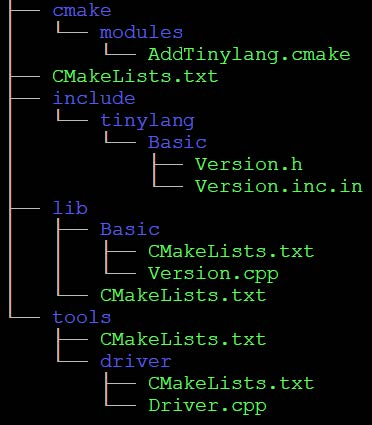
\includegraphics{content/1/chapter2/images/3.jpg}\\
图2.3 – tinylang项目的所有目录和文件
\end{center}

如前所述,有几种方法可以构建tinylang。下面是如何将tinylang构建为LLVM的一部分:\par

\begin{enumerate}
\item 进入构建目录:
\begin{tcolorbox}[colback=white,colframe=black]
\$ cd build
\end{tcolorbox}

\item 执行如下CMake命令:
\begin{tcolorbox}[colback=white,colframe=black]
\$ cmake -G Ninja -DCMAKE\underline{~}BUILD\underline{~}TYPE=Release $\setminus$ \\
\hspace*{1cm}-DLLVM\underline{~}EXTERNAL\underline{~}PROJECTS=tinylang $\setminus$ \\
\hspace*{1cm}-DLLVM\underline{~}EXTERNAL\underline{~}TINYLANG\underline{~}SOURCE\underline{~}DIR=../tinylang $\setminus$ \\
\hspace*{1cm}-DCMAKE\underline{~}INSTALL\underline{~}PREFIX=../llvm-12 $\setminus$ \\
\hspace*{1cm}../llvm-project/llvm
\end{tcolorbox}
通过这个命令,CMake为Ninja(-G Ninja)生成构建文件。构建类型设置为Release,从而生成优化的二进制文件(-DCMAKE\underline{~}BUILD\underline{~}TYPE=Release)。Tinylang作为一个外部项目与LLVM(-DLLVM\underline{~}EXTERNAL\underline{~}PROJECTS=Tinylang)一起构建,源代码位于与构建目录平行的目录中(-DLLVM\underline{~}EXTERNAL\underline{~}TINYLANG\underline{~}SOURCE\underline{~}DIR=../Tinylang)。还提供了构建二进制文件的目标目录(-DCMAKE\underline{~}INSTALL\underline{~}PREFIX=../llvm-12)。最后一个参数指定LLVM项目目录(../llvm-project/llvm)。
	
\item 现在,进行构建和安装:
\begin{tcolorbox}[colback=white,colframe=black]
\$ ninja \\
\$ ninja install
\end{tcolorbox}

\item 构建安装完成后,../llvm-12目录会包含LLVM和tinylang二进制文件。请检查这些应用是否可以运行:
\begin{tcolorbox}[colback=white,colframe=black]
\$ ../llvm-12/bin/tinylang
\end{tcolorbox}

\item 您会看到一些友好的消息。同时,请检查Basic库是否安装:
\begin{tcolorbox}[colback=white,colframe=black]
\$ ls ../llvm-12/lib/libtinylang*
\end{tcolorbox}
这将显示有一个名为libtinylangBasic.a的文件。

\end{enumerate}

当您关注LLVM的开发,并且希望尽快了解API的变化时,使用LLVM进行构建非常有用。第1章中,检查了LLVM的特定版本。因此,没有看到对LLVM源的修改。\par

这里,只构建一次LLVM,然后使用已编译的LLVM版本,将tinylang作为独立项目进行编译:\par

\begin{enumerate}
\item 重新开始,再次进入构建目录:
\begin{tcolorbox}[colback=white,colframe=black]
\$ cd build
\end{tcolorbox}

这一次,CMake仅用于构建LLVM:
\begin{tcolorbox}[colback=white,colframe=black]
\$ cmake -G Ninja -DCMAKE\underline{~}BUILD\underline{~}TYPE=Release $\setminus$ \\
\hspace*{1cm}-DCMAKE\underline{~}INSTALL\underline{~}PREFIX=../llvm-12 $\setminus$ \\
\hspace*{1cm}../llvm-project/llvm
\end{tcolorbox}

\item 与前面的CMake命令比较,除了tinylang的参数没了,其他都一样。
	
\item 创建和安装LLVM与Ninja:
\begin{tcolorbox}[colback=white,colframe=black]
\$ ninja \\
\$ ninja install
\end{tcolorbox}

\item 现在您已经在llvm-12目录中安装了一个LLVM。接下来,将对tinylang项目进行建成。由于它是一个独立的构建,因此需要新的构建目录:
\begin{tcolorbox}[colback=white,colframe=black]
\$ cd ..
\end{tcolorbox}
	
\item 现在创建一个新的build-tinylang目录。Unix上,可以使用以下命令:
\begin{tcolorbox}[colback=white,colframe=black]
	\$ mkdir build-tinylang
\end{tcolorbox}

Windows上,可以使用这个命令:
\begin{tcolorbox}[colback=white,colframe=black]
\$ md build-tinylang
\end{tcolorbox}

\item 任意一个操作系统上用以下命令输入新目录:
\begin{tcolorbox}[colback=white,colframe=black]
\$ cd build-tinylang
\end{tcolorbox}
	
\item 现在运行CMake来创建tinylang的构建文件。唯一的问题是如何发现LLVM,因为CMake不知道LLVM的安装位置。解决方案是指定LLVMConfig.cmake的路径。使用LLVM\underline{~}DIR变量指定该cmake文件所在的文件夹。命令如下:
\begin{tcolorbox}[colback=white,colframe=black]
\$ cmake -G Ninja -DCMAKE\underline{~}BUILD\underline{~}TYPE=Release $\setminus$ \\
\hspace*{1cm}-DLLVM\underline{~}DIR=../llvm-12/lib/cmake/llvm $\setminus$ \\
\hspace*{1cm}-DCMAKE\underline{~}INSTALL\underline{~}PREFIX=../tinylang ../tinylang/
\end{tcolorbox}

\item 安装目录现在也是分开的。构建和安装如下:
\begin{tcolorbox}[colback=white,colframe=black]
\$ ninja \\
\$ ninja install
\end{tcolorbox}

\item 在命令完成后,应该运行../tinylang/bin/tinylang应用程序检查应用程序是否正常。
\end{enumerate}


\hspace*{\fill} \par %插入空行
\textbf{包含LLVM的另一种方法}

如果不想在项目中使用CMake,那么需要找出包含文件和库的位置、要链接的库、使用的构建模式等等。此信息由llvm-config工具提供,该工具位于LLVM安装的bin目录中。假设这个目录包含在shell搜索路径中,可以运行\textit{\$llvm-config}查看所有选项。\par

例如,要让LLVM库链接到支持组件(在前面的示例中使用),可以运行以下命令:\par

\begin{tcolorbox}[colback=white,colframe=black]
\$ llvm-config –libs support
\end{tcolorbox}

输出是一行带有库名的代码,包括编译器的链接选项,例如-lLLVMSupport 、-lLLVMDemangle。显然,这个工具可以很容易地与所选择的构建系统进行集成。\par

有了项目布局,您就有了一个可扩展到大型项目(如编译器)的结构。下一节将介绍另一个基础知识:如何针对不同的目标体系结构进行交叉编译。\par












